A seguir é apresentado uma \textit{timeline} que descreve todas as atividades realizadas durante o período de vigência e que serão realizadas o período pelo bolsista para o desenvolvimento deste projeto. Em seguida, é apresentada uma descrição de cada evento presente na \textit{timeline}. Ressalta-se que todos os artigos que foram publicados durante o período de vigência desse relatório estão destacados tanto na \textit{timeline} quanto na descrição pelo símbolo $\Rightarrow$ ou $\Leftrightarrow$. $\Leftrightarrow$ ilustra capítulo de livro, enquanto o símbolo $\Rightarrow$ refere-se a conferências. Além disso, vale destacar que maiores informações sobre cada evento serão descritas nas seções seguintes.

\begin{itemize}

\item \textbf{Mar 6, 2013 - Jan 20, 2015} - Estudo detalhado sobre ADM e KDM;
\item \textbf{Mar 9, 2013 - Dec 5, 2013} - Implementação de um catalogo de refatoração para o KDM;
\item \textbf{Apr 6, 2013 - Mar 20, 2014} - Realização do Doutorado Sanduíche no INRIA, Lille, França;
\item \textbf{Nov 6, 2013 - Oct 23, 2014} - Elaboração de um metamodelo de refatoração;
\item $\Rightarrow$ Artigo 1 - Concern-Based Refactorings Supported by Class Models to Reengineer Object-Oriented Software into Aspect-Oriented Ones;
\item $\Rightarrow$ Artigo 2 - F3: From features to frameworks;
\item $\Rightarrow$ Artigo 3 - An Approach to Develop Frameworks from Feature Models;
\item $\Rightarrow$ Artigo 4 - F3T: From Features to Frameworks Tool;
\item $\Rightarrow$ Artigo 5 - CCKDM - A Concern Mining Tool for Assisting in the Architecture-Driven Modernization Process;
\item $\Rightarrow$ Artigo 6 - A Combined Approach for Concern Identification in KDM models;
\item $\Leftrightarrow$ Artigo 7 - Developing Frameworks from Extended Feature Models;
\item $\Rightarrow$ Artigo 8 - Evaluating the Effort for Modularizing Multiple-Domain Frameworks towards Framework Product Lines with Aspect-Oriented Programming and Model-Driven Development;
\item $\Rightarrow$ Artigo 9 - Data Network in Development of 3D Collaborative Virtual Environments: A Systematic Review;
\item $\Rightarrow$ Artigo 10 - Towards a Refactoring Catalogue for Knowledge Discovery Metamodel;
\item $\Rightarrow$ Artigo 11 - A Mapping Study on Architecture-Driven Modernization;
\item $\Rightarrow$ Artigo 12 - KDM-AO: An Aspect-Oriented Extension of the Knowledge Discovery Metamodel;
\item $\Rightarrow$ Artigo 13 - Investigating Lightweight and Heavyweight KDM Extensions for Aspect-Oriented Modernization;
\item $\Rightarrow$ Artigo 14 - KDM-RE: A Model-Driven Refactoring Tool for KDM;

\item \textbf{16/2/2015 - 19/2/2016} - Esse período representa as Etapas Seguintes;

\begin{itemize}
	\item \textbf{7/3/2015 - 8/7/2015} - Elaboração de Artigos;
	\item \textbf{15/5/2015 - 28/11/2015} - Implementar Refatorações Arquiteturais;
	\item \textbf{28/5/2015 - 30/09/2015} - Estudo Experimental;
	\item \textbf{29/06/2015 - 3/11/2015} - Redação da Tese;
	\item \textbf{08/09/2015 - 10/01/2016} - Evolução Ferramental;
	\item \textbf{Fevereiro} - Defesa do Doutorado;
\end{itemize}

\end{itemize}


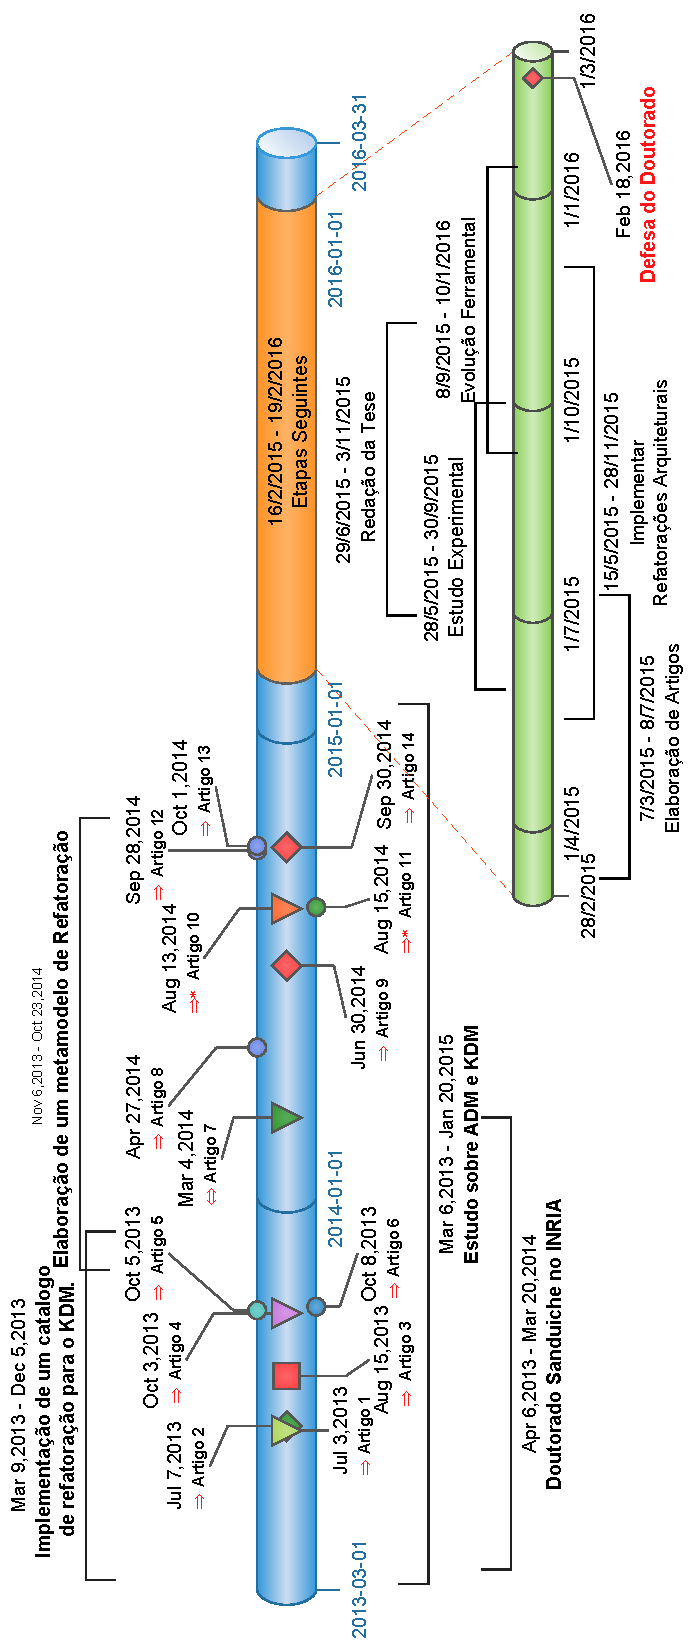
\includepdf[pages={-}]{figuras/timeLine}